\chapter{Pruebas Realizadas} \label{cap:nueve}
\section{Pruebas Dinámicas}

La pruebas dinámicas son todas aquellas pruebas que para su realización requieren la ejecución de la aplicación. Las pruebas dinámicas permiten el uso de técnicas de caja negra y caja blanca con mayor amplitud. Debido a la naturaleza dinámica de la ejecución de pruebas es posible medir con mayor precisión el comportamiento de la aplicación desarrollada.\\

Dentro de las pruebas dinámicas podemos encontrar distintos niveles de prueba. Los niveles de prueba son grupos de actividades de prueba que se organizan y gestionan juntas. Cada nivel de prueba es una instancia del proceso de prueba, realizadas en relación con software en un determinado nivel de desarrollo, desde unidades individuales o componentes hasta sistemas completos o, en su caso, sistemas de sistemas.\\

Los niveles de prueba utilizados pueden ser:

\begin{itemize}
	\item Prueba de componentes.
	\item Pruebas de integración.
	\item Prueba de sistema.
	\item Pruebas de aceptación.
\end{itemize}

Los niveles de prueba se caracterizan por los siguientes atributos:

\begin{itemize}
	\item Objetivos específicos
	\item Base de prueba, referenciada para derivar casos de prueba
	\item Objeto de prueba (es decir, lo que se está probando)
	\item defectos y fallas típicas
\end{itemize}

\subsection{Prueba de sistema}

\textbf {Objetivos de las pruebas del sistema.}\\

Las pruebas del sistema se centran en el comportamiento y las capacidades de un sistema o producto completo, a menudo considerando las tareas de extremo a extremo que el sistema puede realizar y los comportamientos no funcionales que exhibe mientras realiza esas tareas. Los objetivos de las pruebas del sistema incluyen:

\begin{itemize}
	\item Reducción del riesgo.
	\item Verificar si los comportamientos funcionales y no funcionales del sistema son los diseñados y
	especificado
	\item Validar que el sistema está completo y funcionará como se esperaba.
	\item Generar confianza en la calidad del sistema en su conjunto.
	\item Encontrar defectos
	\item Evitar que los defectos escapen a niveles de prueba o producción más altos
\end{itemize}

\textbf {Base de prueba}\\
Los ejemplos de productos de trabajo que se pueden usar como base de prueba para las pruebas del sistema incluyen:

\begin{itemize}
	\item Especificaciones de requisitos del sistema y software (funcionales y no funcionales)
	\item Informes de análisis de riesgos.
	\item Casos de uso
	\item Epics e historias de usuarios
	\item Modelos de comportamiento del sistema.
	\item Diagramas de estado
	\item Sistema y manuales de usuario.
\end{itemize}

\textbf {Objetos de prueba}\\
Los objetos de prueba típicos para las pruebas del sistema incluyen:

\begin{itemize}
	\item Aplicaciones
	\item Sistemas de hardware / software
	\item Sistemas operativos
	\item Sistema bajo prueba (SUT)
\end{itemize}

\hspace{.85cm}

\subsubsection{REPORTE DE PRUEBAS SPRINT 1 - CICLO 1}

Las pruebas contempladas para el primer ciclo de pruebas abarcan los Casos de Uso del Sprint 1, Los cuales comprenden las siguientes gestiones:

\begin{itemize}
	\item CU1 Iniciar sesión.
	\item CU2 Gestionar proyectos de Administrador.
	\item CU3 Gestionar Colaboradores.
	\item CU4 Gestionar Proyectos de Colaborador.
\end{itemize}

Se realizaron pruebas dinámicas de sistema, con técnicas de caja negra.\\

Base de prueba:
\begin{itemize}
	\item Casos de Uso
	\item Especificaciónes de requisitos del sistema y software.
	\item Sistema y manual de usuario.
\end{itemize}

Objeto de prueba:
\begin{itemize}
	\item Sistema de software
\end{itemize}

\newpage

Los resultados finales del primer ciclo de prueba arrojaron los siguientes datos:

\begin{figure}[H]
	\begin{center}
		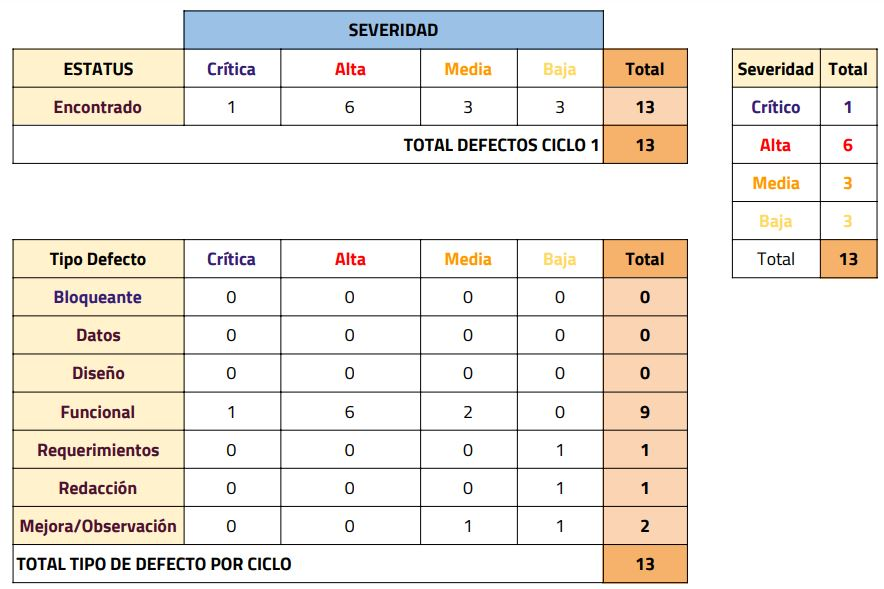
\includegraphics[width=.95\textwidth]{images/pruebas/s1c1}
		\caption{Informe de defectos Sprint 1 Ciclo 1}
		\label{fig:infos1c1}
	\end{center}
\end{figure}

\newpage

\begin{figure}[H]
	\begin{center}
		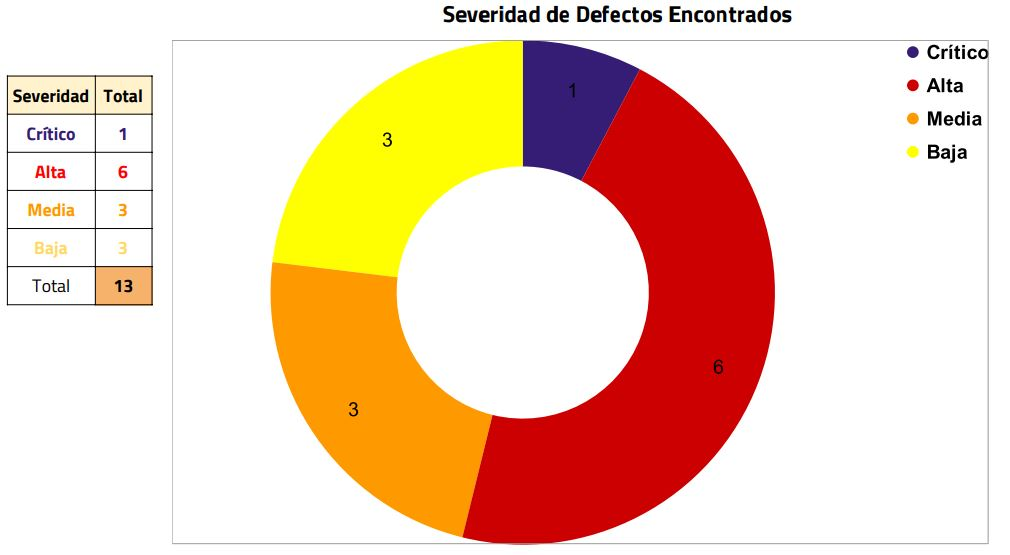
\includegraphics[width=.85\textwidth]{images/pruebas/s1c1-1}
		\caption{Gráfica de defectos por severidad Sprint 1 Ciclo 1}
		\label{fig:infos1c1-1}
	\end{center}
\end{figure}

\begin{figure}[H]
	\begin{center}
		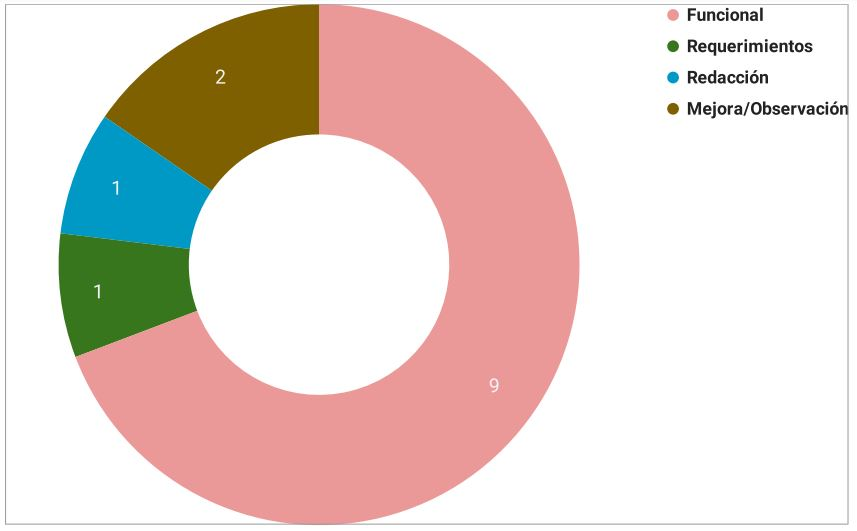
\includegraphics[width=.75\textwidth]{images/pruebas/s1c1-2}
		\caption{Gráfica de defectos por tipo de defecto Sprint 1 Ciclo 1}
		\label{fig:infos1c1-2}
	\end{center}
\end{figure}

\newpage

\begin{figure}[H]
	\begin{center}
		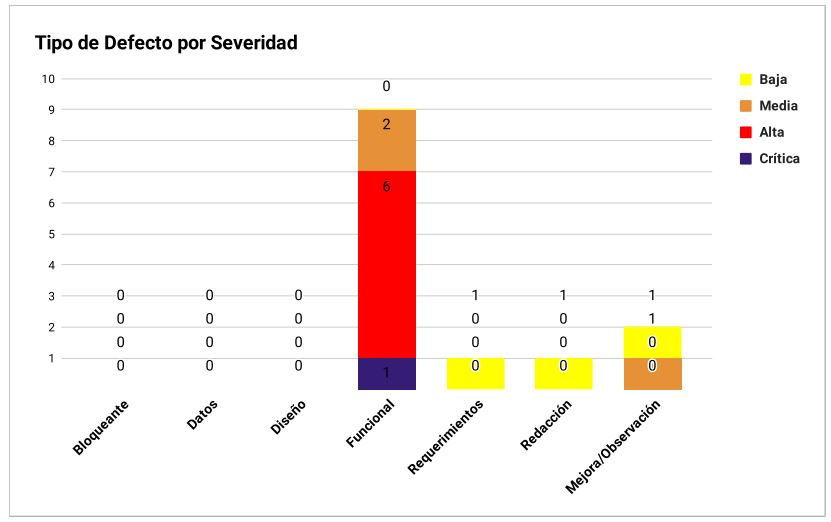
\includegraphics[width=.95\textwidth]{images/pruebas/s1c1-3}
		\caption{Gráfica de tipo de defectos por severidad Sprint 1 Ciclo 1}
		\label{fig:infos1c1-3}
	\end{center}
\end{figure}

Se corrigieron los defectos encontrados en el primer ciclo.
